%Goals
%Sie kennen das Konzept von Klassen und Structs in C#
%Sie kennen den Parameterübergabe-Mechanismus von C#
%Sie können Properties und indexers
%Sie kennen das Konzept des Operator-Overloadings
%Sie könnne die gelernten Konzepte in praktischen Progammieraufgaben anwenden

\section{Klassen und Structs}
\subsection{Klassen}
Sind Referenz Typen und werden auf dem Heap angelegt.

\textbf{Vererbung}\\ 
Ableiten von Basisklasse möglich, Verwenden als Basisklasse möglich, Implementieren von Interfaces möglich.

\textbf{Felder} \\
Eine Konstante einer Klasse muss zur Compilezeit berechenbar sein. Ein "readonly" Feld darf zur Laufzeit nicht mehr geändert werden. 

\textbf{Nested Types} \\
Sind für spezifische Hilfsklassen gedacht. Die äussere Klasse hat Zugriff auf innere KLasse (Nur Public). Die innere Klasse hat Zugriff auf äussere Klasse (auch private!).

\textbf{Statische Klassen} \\
Regeln: Nur statische Members erlaubt, kann nicht instanziert werden, sind "sealed".

\textbf{Statische Usings} \\
Verkürzen den Quellcode bei Verwendung von statischen Klassen. Regeln: Nur statische Klassen sowie Enums erlaubt. Importiert alle: statischen Members, Statischen Nested Members. Namenskonflikte: Normale Namensauflösungsregeln wie bei überladenen Methoden, bei identischen Signaturen muss Klassenname vorangestellt werden..

\begin{lstlisting}
class Stack {
	const long = 12; // Konstante muss zur Compilezeit berechenbar sein
	int[] values;
	int top = 0;
	public Stack(int size) { /* ... */ }
	public void Push(int x) { /* ... */ }
	public int Pop() { /* ... */ } }
}
Stack s = new Stack(10); 
\end{lstlisting}

\subsubsection{Partielle Klassen}
Das partial Keyword erlaubt die Definition in mehreren Files. Es sind auch partielle Methoden möglich. Regeln: "partial" muss bei allen Teilen angemerkt sein, Alle Teile müssen das gleiche Sichtbarkeitsattribut haben. Es gibt auch partielle Methoden.
\begin{lstlisting}
// File1.cs 
partial class MyClass {
public void Test1() { } } 
// File2.cs 
partial class MyClass {
public void Test2() { } }
// Verwendung 
MyClass mc = new MyClass(); 
mc.Test1(); 
mc.Test2();

\end{lstlisting}

\subsubsection{Abstrakte Klassen}
Eine Mischung aus Klasse und Interface. Deklaration mit dem Schlüsselwort "abstract". Regeln: Kann nicht direkt instanziert werden, Kann beliebig viele Interfaces implementieren, Alle Interface-Members müssen deklariert werden, Abgeleitete (nicht abstrakte) Klassen müssen alle abstrakten Members implementieren, Abstrakte Members können nur innerhalb abstrakter Klassen deklariert werden, Dürfen nicht «sealed» (versiegelt) sein (siehe später).

\begin{lstlisting}

\end{lstlisting}

\subsection{Structs}
Sind Value types und werden auf dem Stack oder "in-line" in einem Objekt auf dem Heap abgelegt.

\textbf{Vererbung} \\
Ableiten von Basisklasse nicht möglich, Verwenden als Basisklasse auch nicht möglich, Implementieren von Interfaces ist möglich.

\textbf{Felder} \\
Felder dürfen im Struct nicht initialisiert werden!

\begin{lstlisting}
struct Point {
	int x;
	int y;
	public Point(int x, int y)
	{
	this.x = x; this.y = y; 
	} 
	public void MoveX(int x) { /* ... */ } 
	public void MoveY(int y) { /* ... */ }
}
Point p = new Point(2, 3); 
\end{lstlisting}

\textbf{Verwendung} \\
Ein Struct sollte nur unter folgenden Umständen verwendet werden. In allen anderen Fällen sollte eine Klasse verwendet werden.
\begin{itemize}
  \itemsep -0.5em 
  \item Repräsentiert einen einzelnen kleinen Wert
  \item Instanzgrösse ist kleiner als 16 Byte
  \item Ist immutable
  \item Wird nicht häufig geboxt
  \item Ist entweder: kurzlebig, eingebettet in anderes Objekt
\end{itemize}

\subsection{Properties}
Properties sind eine Kurzform für Get-/Set-Methoden. Diese können für Structs und Klassen eingesetzt werden. Sind ein reines Compiler-Konstrukt. Nutzen: Benutzersicht/Implementation können unterschiedlich sein, Validierung beim Zugriff, Ersatz für Public Fields auf den Interfaces, Über Reflection als Property identifizierbar. Private properties können nur von der Klasse selbst verwendet werden.
\begin{lstlisting}
class MyClass {
	private int length; // Backing field
	// Property
	public int Length {
		get { return length; }
		set { length = value; }
	}
	// Compiler Output
	public int get_Length() { return length; } 
	public void set_Length(int value) { length = value; }
\end{lstlisting}

\subsection{Auto-Implemented Properties}
Das Backing field sowie die Setter und Getter werden automatisch generiert. Für jede abweichende Get-/Set-Logik muss Property explizit implementiert werden.
\begin{lstlisting}
// Auto Property - backing filed gets generated automatically
public int LengthAuto { get; set; }
public int LengthInitializes {get; /* set; */ };
\end{lstlisting}

\subsection{Initialisierte Properties}
Properties können bei der Objekt Erstellung direkt initialisiert werden. Das ist ein reines Compiler-Feature.
\begin{lstlisting}
MyClass mc = new MyClass()
{
	Length = 1, 
	Width = 2
};
// Compiler Output
MyClass mc = new MyClass();
mc.Length = 1;
mc.Width = 2;
\end{lstlisting}

\subsection{Indexer}
Indexer ermöglichen, dass Instanzen einer Klasse oder Struktur wie Arrays indiziert werden. Der indizierte Wert kann festgelegt oder ohne explizite Angabe eines Typs oder Instanzmembers abgerufen werden. Indexer ähneln Eigenschaften. Der Unterschied besteht jedoch darin, dass ihre Zugriffsmethoden Parameter verwenden. Das Schlüsselword this definiert den Indexer. Das Schlüsselwort value für Zugriff auf Wert in Setter.
\begin{lstlisting}
class SampleCollection<T> {
   private T[] arr = new T[100];
   // Define the indexer to allow client code to use [] notation.
   public T this[int i] {
      get { return arr[i]; }
      set { arr[i] = value; }
   }
}
class Program
{
   static void Main() {
      var stringCollection = new SampleCollection<string>();
      stringCollection[0] = "Hello, World";
      Console.WriteLine(stringCollection[0]);
   }
}
\end{lstlisting}

\subsection{Konstruktoren}
Bei jedem Erzeugen einer Klasse / eines Structs verwendet (Aufruf von «new»).

\begin{minipage}{0,5\linewidth}
\textbf{Default-Konstruktor Klasse}
\begin{itemize}
  \itemsep -0.5em 
  \item Automatisch generiert, wenn nicht vorhanden
  \item Wenn anderer Kstr. vorhanden nicht mehr
  \item Kann manuell implementiert werden
  \item Initialisiert Felder mit default(T)
  \item Kann beliebig viele Felder initalisieren
\end{itemize}
\end{minipage}
\begin{minipage}{0,5\linewidth}
\textbf{Default-Konstruktor Klasse}
\begin{itemize}
  \itemsep -0.5em 
  \item Wird immer automatisch generiert!
  \item Kann nicht manuell definiert werden
  \item Initialisiert Felder mit default(T)
  \item Muss alle Felder initialisieren!
\end{itemize}
\end{minipage}

\begin{figure}[h!]
	\centering
  	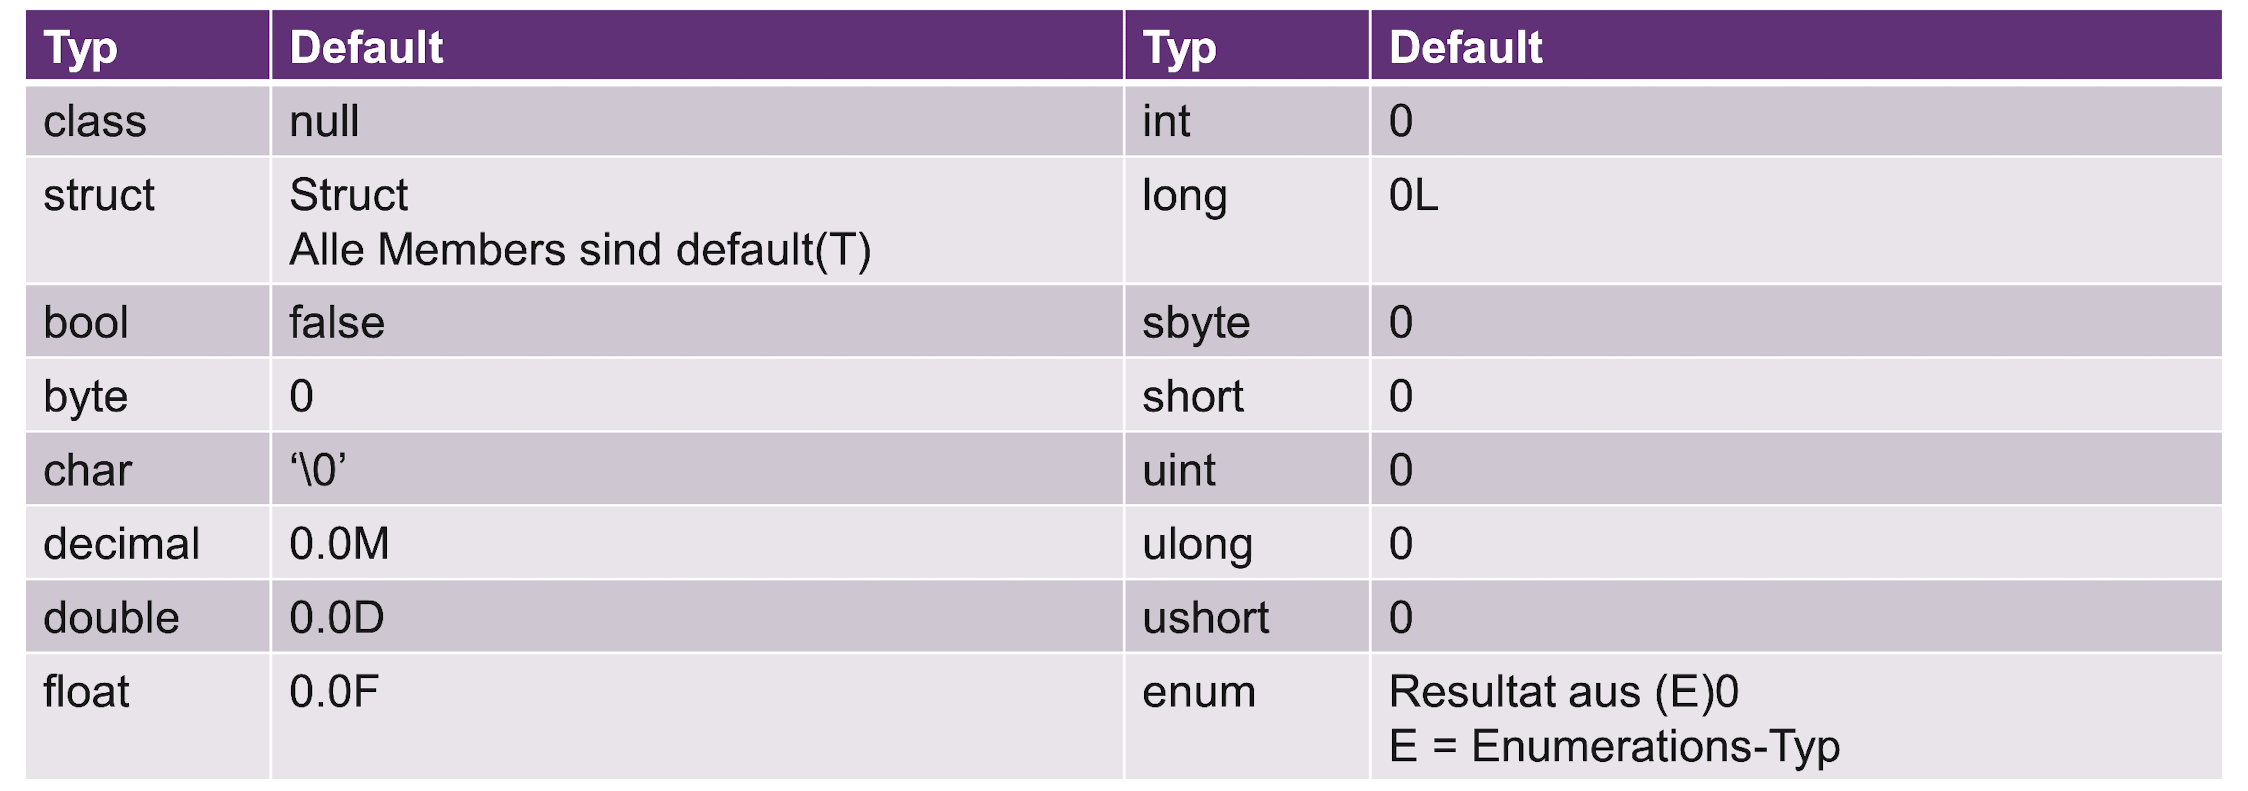
\includegraphics[width=0.75\textwidth]{standardwerte}
    \caption{Standard-Werte}
\end{figure}

\subsubsection{Statische Konstruktoren}
Für statische Initialisierungsarbeiten verwendet und sind identisch für die Klasse und Struct. Regeln: zwingend Parameterlos, Sichtbarkeit darf nicht angegeben werden, Wird genau einmal ausgeführt, Kann nicht explizit aufgerufen werden.

\subsubsection{Dekonstruktoren}
Ermöglichen Abschlussarbeiten beim Abbau eines Objekts (wie Java-Finalizer) Regeln: Nur bei Klassen erlaubt, Zwingend Parameterlos/Sichbarkeitslos, Maximal einer erlaubt, Wird vom Garbage Collector aufgerufen und kann nicht explizit aufgerufen werden.
\begin{lstlisting}
class MyClass {
	~MyClass() {
		// Freigabe von File-Handles etc.
	}
}
\end{lstlisting}

\subsubsection{Initalisierungs-Reihenfolge}
%TODO add initalisierungsreihenfolge

\subsection{Operatoren - Überladung}
%TODO add Operatorenüberladung

\pagebreak


\section{Methoden}
\subsection{Statische Methoden}
Es gibt zwei Ausprägungen von statischen Methoden: Prozedur (Aufgabe ohne Rückgabewert), Funktion. 

\subsection{Value Parameter}
Kopie des Inhalts wird übergeben (Wert oder Heap-Referenz).
\begin{lstlisting}
void IncVal(int x) { x = x + 1; } 
void TestIncVal() {
	int value = 3;
}
IncVal(value); // value == 3 
\end{lstlisting}

\subsection{Reference Parameter}
Adresse der Variable wird übergeben. Variable muss initialisiert sein. Es muss eine Variable übergeben werden. Hierfür wird das ref keyword verwendet.
\begin{lstlisting}
void IncRef(ref int x) { x = x + 1; } 
void TestIncRef() {
	int value = 3;
IncRef(ref value); // value == 4
\end{lstlisting}

\subsection{Out-Parameter}
Werden wir ref-Parameter verwendet, aber sind für die Initialisierung gedacht. Das bedeutet, dass die Variable vorher nicht initialisiert werden muss. Das out keyword muss beim Aufrufer und in der Methode deklariert werden.
\begin{lstlisting}
static void Init(out int val) {
	val = 100;
}
int value;
Init(out value);	
\end{lstlisting}

\subsection{In Parameter}



\subsection{Params-Array}
Erlaubt beliebig viele Parameter. Muss am Schluss der Deklaration stehen. Nur ein params-Array ist erlaubt. Darf nicht mit ref oder out kombiniert werden.
\begin{lstlisting}
void Sum(out int sum, params int[] values) {
	sum = 0;
	foreach (int i in values) sum += i; 
} 
\end{lstlisting}

\subsection{Optionale Parameter (Default Values)}
Optionale Parameter ermöglichen die Zuweisung eines Default-Values. Deklaration muss hinter der erforderlichen Parameter erfolgen! Muss zur Compilezeit berechenbar sein.
\begin{lstlisting}
private void Sort(int[] array, int from=0, bool ascending=true) { /* . */ }
\end{lstlisting}

\subsection{Named Parameter}
Identifikation der optionalen Parameter anhand des Namens (anstatt anhand der Position). 
\begin{lstlisting}
Sort(a, ignoreCase: true, from: 3);
\end{lstlisting}

\subsection{Überladung}
Mehrere Methoden mit dem gleichen Namen möglich. Voraussetzung: Unterschiedliche Anzahl Parameter oder Parametertypen oder Parameterarten (ref/out). \textit{Der Rückgabetype spielt dabei keine Rolle!}
\begin{lstlisting}
void Test(int x) { /* ... */ } 
void Test(char x) { /* ... */ } 
void Test(int x, long y) { /* ... */ } 
void Test(long x, int y) { /* ... */ } 
void Test(ref int x) { /* ... */ }
\end{lstlisting}


%TODO add operatoren

\subsection{Lamda Expressions}
\begin{itemize}
  \itemsep -0.5em 
  \item Eine Lambda Expression ist eine anonyme Methode
 	\SubItem{Keine Implementation einer benannten Methode nötig}
 	\SubItem{Kein "delegate" Schlüsselwort nötig}
 	\SubItem{Angabe von Parametertypen ist optional}
  \item Ist die Basis für das Erzeguen von Delegates und Expression Trees.
  \item Zwei Ausprägungen: Expression Lambdas, Satement Lambdas.	
  \item Werden in Delegates konvertiert
\end{itemize}

\begin{lstlisting}
// Expression Lambda 
Func<int, bool> fe = i => i % 2 == 0;
// Statement Lambda 
Func<int, bool> fs = i => {
	int rest = i%2; 
	bool isRestZero = rest == 0; 
	return isRestZero;
};
\end{lstlisting}

%TODO extend lambdas
\pagebreak
